\chapter{\label{method}Improving the Bucket with Global\\Query-algorithm}

\todo{This chapter have sections to be completed is apparently quite messy. Content-wise it is fairly complete.}

\section{Background}

\textbf{The Company}  Something about a a very common business model (small startup, free-to-play) limited budget and business not large enough to run server park on its own.

\textbf{The Application} Game, number of users

\textbf{Infrastructure} The backend handling the highscores and rankings runs on Google App Engine (GAE) which is a Platform-as-a-Service-cloud service (PaaS). The current system is implemented in Java.

Since applications running on GAE do not have access to a file system, data is stored in the App Engine Datastore which is NoSQL key-value-store. While the application part of the GAE scales automatically as far as the configuration allows, the throughput when writing to the same object in the Datastore is very limited and measures need to be taken to avoid cogestion. 

Finally a service provided by the GAE worth mentioning is the memory cache. The Memory cache or memcahce is provided at different service levels, paid and free, the later without any guarantees at all. The memcache may be used for keeping the number of reads from the datastore at a minimum. It is however not durable and cache-misses needs to be handled gracefully.

\section{Problem description revisited}

The Companys current ranking algorithm is an implementation of the algorithm \emph{Bucket with Global Query} (See \labelcref{bucket}). The highscores are stored in Google App Engines Datastore as entities with properties \emph{username} and a \emph{highscore}. When a player gets a new highscore it replaces the old highscore. Note that this implies that highscore entries never will get updated with a lower score than previously recorded for that user.

Since score in this case is measured in milliseconds and lower timings are better a better score is a lower number\footnote{While this really should not matter at all, be aware that this fact is a good foundation for getting mindfucked very hard}.

\section{Hypothesis} 

The current implementation starts a background job that builds the bucket-table every ten minutes. When the scan is complete a reference is set to the new table and the old one is discarded. The error is a priori assumed to be at its maximum level right before the switch (See figure \ref{fig:errortime}) and will in the forthcoming reasonings serve as an upper limit for what would be an acceptable performance.

The total cost for providing the ranking service with the current implementation and the implementation to be assessed is

\begin{equation}
  n \times C_{estimate} + \frac{ C_{table}}{n}
\end{equation}

where $n$ is the number of approximations made, $C_{estimate}$ is the execution time for making one estimate and $C_{table}$ is the cost for recreating the bucket-table.
\todo{Create better formula. Maybe total cost = function(num-estimates, table-recreation-frequency, cost-estimate, cost-table-recreation)}

In the original Bucket with Global Query-algorithm, getting an approximate rank is a lookup-operation in a table (or similar operation on another data structure) and some simple arithmetics. Hence the execution time cannot really be improved for that part.

The cost for creating a bucket-table can not be radically improved either, but if the lifetime of the bucket-table could be extended, its addition to the cost per rank estimate would get lower [XXXX]. As shown in section \ref{bucket}, the bucket-table in use starts to deviate from a true bucket-table when new highscores comes in. The tables score ranges, start ranks and bucket sizes simply don not correspond to the actual set of highscores.

So what if the table's buckets were adjusted when a new highscore gets registered? Adjusting start ranks and bucket sizes will be reasonably fast, but there is also an overhead storing the adjusted table which would apply to every single estimate.

\todo{Improve or remove}

\begin{equation}
  n \times C_{estimate} \times C_{update} + \frac{ C_{table}}{n}
\end{equation}

To sum up, the cost for approximating the rank for a highscore will be more expensive when also updating the bucket-table, but will the increased cost it be compensated for by the expected increase in lifetime of the bucket-table? The cost for recreating the bucket table will remain the same. Two possible scenarios are sketched in figure \ref{fig:cost}.

\begin{figure}[h]
  \centering
  \caption{Possible scenarios for cost growth.}
  \label{fig:cost}
  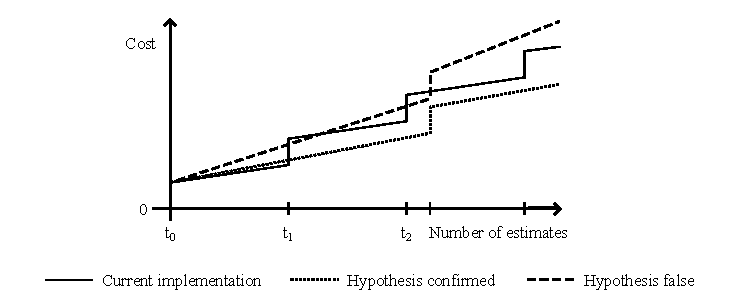
\includegraphics[width=13cm]{img/hypothesis-cost1.eps}
\end{figure} 

The hypothesis reads as follows: \emph{\textbf{Running the ranking service with the new implementation will be more efficient than the current implementation at the same level of error.}}

\section{Data}

In this experiment only synthetic data will be used. The choice is both practical and a methodologically motivated. First, the production system as cannot be altered in such a way that real world data could be tapped within this experiments timeframe. Also, real world data in this system differs from one time period to another both in terms of the highscore distribution and throughput -- and of course, data from one application differs from data from other applications. Using synthetic data make the results more general.

The experiment is started with a random set of highscores which have a Gaussian distribution with mean 1 000 000 and variance 1 000 000, also scores below 1000 are not included\footnote{The real world highscores are similarly distributed to each other and somewhat similar to a Gaussian distribution. However, no effort has ben made to do a statistical analysis of them.} (See figure \ref{fig:highscore-distribution}).
 
\begin{figure}[h]
  \centering
  \caption{Initial highscore distribution.}
  \label{fig:highscore-distribution}
  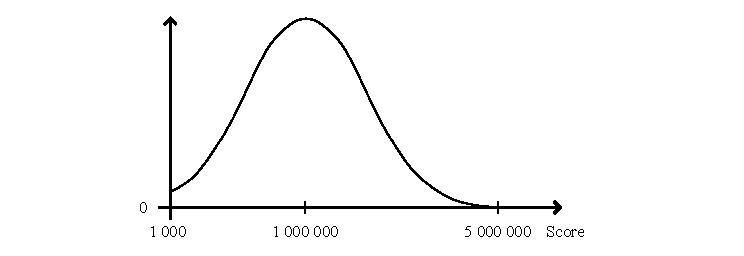
\includegraphics[width=13cm]{img/highscore-distribution.eps}
\end{figure} 

When the experiment is running, highscores are picked at random, and gets a better score, picked from a uniform distribution $\mathcal{U}\{1, 1000\}$.

The random number generator in Java is used, but is always initialized with the same random seed to achieve repeatability.  

\section{What and how to measure}

To be able to test the hypothesis relative error and execution time will be logged per ranking request.

For the \emph{true} value for calculating the relative error, an exact rank is calculated for that instant. While using other values as true values, such as values created with a fresh bucket-table every time, the exact value seemed to be the most predictable option.

The execution time is measured by calls to \texttt{System.currentTimeInMillis()} in the servlet receiving the ranking request.

\section{The experiment}

\todo{Illustration?}

The experiment is implemented in a client-server-model where the client simulate playing a game and sends highscores to the server. The server responds with an estimated rank and the execution time for processing the request. The client is a regular Java program with no bells and whistles and the server consists of a number of servlets designed to run on Google App Engine. 

When the client has finnished ``playing'' a round it always get a new highscore, ie it always wins. The new highscore is better than the old one by a number drawn from a uniform pseudorandom distribution $1-1000$.

To be able to measure the relative error of the estimates the client starts by asking for a list of all highscores. When the client sends a new highscore to the server it also updates its local highscore list. When the server responds with the rank estimate for the new score, that estimate is compared with the real rank and ultimately used for calculating the relative error.

The type of ranking algorithm to use is set before starting the test.


\subsubsection{Libraries}

A few libraries are used; \emph{Objectify} which provides means for persisting Java objects to the App Engines Datastore
and \emph{Jackson} for parsing and generating JSON-data. Naturally, the App Engine SDK is also used.

\todo{Make list and references}

\section{Limitations}

\todo{The real world data set grows over time. Will be ignored, only focus on case when the set of highscores are reasonably large.}

\todo{Only tested on development server}

\todo{Rest of chapter cut from introduction}

